
\subsection{Coevaluation}
When dealing with a construction in category theory, it is natural to
simultaneously study its dual, that is the construction obtained by
\emph{reversing all the arrows}. If in definition \ref{def:eval} we
substitute the product $\prod^nR$ by its dual $\coprod^nR$, called
\emph{coproduct}, we obtain a new way of evaluating an arithmetic
circuit that we will call \emph{coevaluation}. We study here the
properties of coevaluation, its interest will be clear in the next
sections.

In this context, we will make an abuse by using the same notation
$R^n$ we used for the product to signify the coproduct $\coprod^nR$ in
the category. Whether $R^n$ is product or coproduct will always be
clear from the context.

\begin{definition}[Arithmetic co-operator, cobasis]
  Let $R$ be a ring. An arithmetic co-operator over $R$ is a function
  $f:R^i\ra R^o$ for some $i,o\in\N$; here $R^n$ is coproduct.

  An arithmetic $R$-cobasis is a set of arithmetic co-operators over
  $R$.
\end{definition}

In particular when the category is $\mathsf{Set}$ the coproduct is the
disjoint union of sets, thus the bases $\Sbasis$ and $\Tbasis$ make no
sense in this context.

The definitions of node and circuit naturally extend to cobases, but
we need to define a new evaluation for arithmetic circuits defined
over them.

\begin{definition}[coevaluation of an arithmetic circuit]
  \label{def:coeval}
  Let $C$ be an arithmetic circuit with $i$ inputs and $o$ outputs
  over a cobasis $\mathcal{B}$. Its coevaluation is a function
  $\lave_C:R^i\ra R^o$.

  We use the same notation as in definition \ref{def:eval}. As we did
  there, we simultaneously define $\lave_v$ for each $v\in V$ and
  $\lave_e$ for each $e\in E$.
  \begin{itemize}
  \item Let $v\in V$ have in-degree $m$, let its coevaluation be
    $\lave_v:R^m\ra R^o$ and let $\iota_1,\ldots,\iota_n$ be the
    canonical injections from $R$ to $R^m$. Let $i_1<_v\cdots<_vi_m$
    be the input ports of $v$ and let
    $e_j=\bigl(i_j,E^{-1}(i_j)\bigr)$ be the corresponding edges
    incident to $v$, then $\lave_{e_j} = \lave_v\circ\iota_j$ for any
    $j$.
  \item Let $y_1<_V\cdots<_Vy_n$ be the output nodes and let
    $\iota_1,\ldots,\iota_o$ be the canonical injections from $R$ to
    $R^o$, then $\lave_{y_j}=\iota_j$ for any $j$.
  \item For every evaluation node $v$ with out-degree $n$, let
    $o_1<_v\cdots<_vo_n$ be the output ports of $v$ and let
    $e_j=\bigl(E(o_j),o_j\bigr)$ be the corresponding edges
    stemming from $v$, then
    \begin{equation}
      \label{eq:lave_v}
      \lave_v = (\lave_{e_1} \oplus \cdots \oplus \lave_{e_n}) \circ \beta(v) 
      \text{.}
    \end{equation}
  \item For every input node $x$, let $e\in E$ be the only edge
    stemming from $x$, then $\lave_x=\lave_e$.
  \end{itemize}

  We can finally define $\lave_C:R^i\ra R^o$. Let $x_1<_V\cdots<_Vx_i$
  be the input nodes, then
  \begin{equation}
    \label{eq:lave}
    \lave_C = \lave_{x_1} \oplus \cdots \oplus \lave_{x_i}
    \text{.}
  \end{equation}
\end{definition}

As before, the sums of equations \eqref{eq:lave_v} and \eqref{eq:lave}
are formally defined via the universal property of the coproduct.

The coevaluation in general does not attach the same semantics to a
circuit as the evaluation. For example in the case of $\mathsf{Set}$
the coevaluation is a function from the disjoint union of $i$ copies
of $R$ to the disjoint union of $o$ copies of $R$. We can regard
circuits over cobases in $\mathsf{Set}$ as objects that are fed one
single element of $R$ on one out of their $n$ inputs and then take
decisions depending on which input was fed. An example is given in
figure \ref{fig:coffee}.

\begin{figure}[!ht]
  \centering
  
  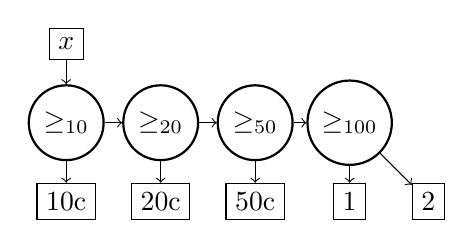
\begin{tikzpicture}
    \tikzstyle{node}=[circle,thick,draw=black,minimum size=4mm]
    \tikzstyle{arg}=[rectangle,thin,draw=black,minimum size=4mm]

    \begin{scope}
      \node[arg](in){$x$};

      \node[node,below of=in](s10){$\ge_{10}$};

      \node[node,right of=s10,xshift=2mm](s20){$\ge_{20}$};
      \node[arg,below of=s10](o10){$10$c};

      \node[node,right of=s20,xshift=2mm](s50){$\ge_{50}$};
      \node[arg,below of=s20](o20){$20$c};

      \node[node,right of=s50,xshift=2mm](s1){$\ge_{100}$};
      \node[arg,below of=s50](o50){$50$c};

      \node[arg,below of=s1](o1){$1$\euro};
      \node[arg,right of=o1](o2){$2$\euro};

      \path[->]
      (in) edge (s10)
      (s10) edge (o10)
      (s10) edge (s20)
      (s20) edge (o20)
      (s20) edge (s50)
      (s50) edge (o50)
      (s50) edge (s1)
      (s1) edge (o1)
      (s1) edge (o2);
    \end{scope}
  \end{tikzpicture}  
  
  \caption{The coffee machine circuit. On input $r\in R$, the operator
    $\ge_x:R\ra R\uplus R$ gives $r$ on its first output if $r\ge x$, on its
    second output otherwise. The circuit is an euro coin separator.}
  \label{fig:coffee}
\end{figure}

In some cases, howevever, evaluation and coevaluation coincide. The
following lemma shows one important case when this happens.

\begin{lemma}
  \label{th:coeval}
  Let $C$ be a circuit over $(R,\Tbasis)$. In the category $RMod{R}$
  $\eval_C\simeq\lave_C$.
\end{lemma}
\begin{proof}
  For finite dimensional modules, the product and the direct sum are
  the same object. More formally, when working in $RMod{R}$ there is
  a natural isomorphism $\prod^n R\simeq\coprod^n R$ for any $n$ (this
  is true for any additive category, see \cite[VIII.2]{McLane}). Thus
  $\Tbasis$ is both a basis and a cobasis, up to isomorphism, and both
  evaluation and coevaluation of circuits over it are meaningful.

  The rest of the proof is just induction on the size of the
  circuit. First, it is obvious that for elementary circuits with an
  unique evaluation node $v$ we have $\eval_C \simeq \beta(v) \simeq
  \lave_C$. Then it suffices to show that the property is maintained
  upon composition of circuits.
\end{proof}

The equivalence of evaluations and coevalutions suggests that there is
some unexploited symmetry in circuits over $\Tbasis$. The next
section explores it.




% Local Variables:
% mode:flyspell
% ispell-local-dictionary:"american"
% mode:TeX-PDF
% mode:reftex
% TeX-master: "../these"
% End:
%
